\subsection{a}
\begin{figure}[h]
	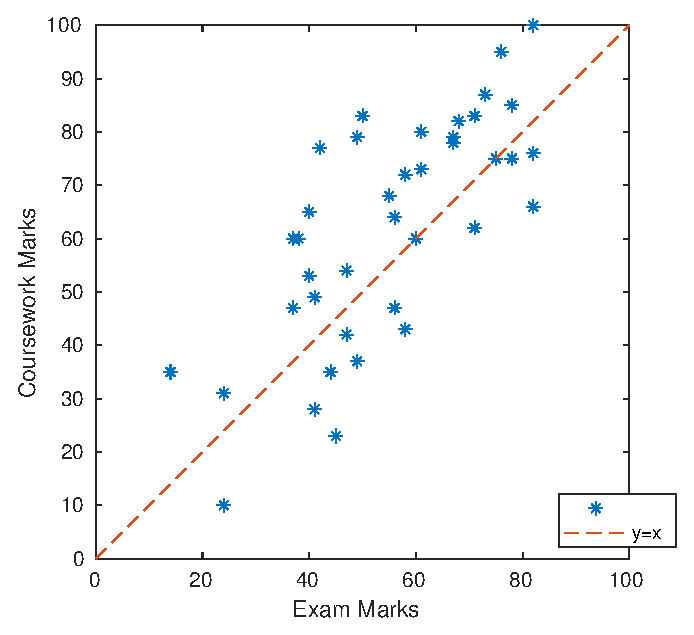
\includegraphics[scale=0.6, center]{./eps/topic1_a.eps}
    \caption{Coursework marks plotted against exam marks. Note the orange dashed line of symmetry}
    \label{fig:Topic1-a}
\end{figure}
In Figure \ref{fig:Topic1-a} the line of symmetry, $x=y$, was plotted.
Because the data are reasonably spread around the line of symmetry, there is evidence for some proportionality between the two data sets.
\lstinputlisting[caption={Code for Topic 1. Question a.}]{"./files/topic 1/a.m"}

\pagebreak

\subsection*{b}
\begin{figure}[h]
	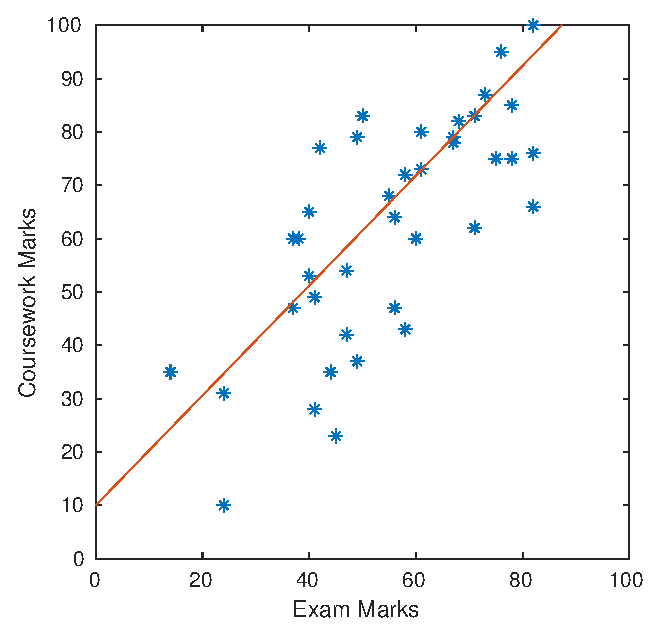
\includegraphics[scale=0.6, center]{./eps/topic1_b.eps}
	\caption{Coursework marks plotted against exam marks. Line of best fit estimated by eye}
	\label{fig:Topic1-b}
\end{figure}
Given a line $y=ax+b$, the parameters were estimated as per below. This is represented in Figure \ref{fig:Topic1-b}.
\begin{equation}
\begin{split}
	a &= \frac{90-10}{78-0} = 1.03 \\
	b &= 10
\end{split}
\end{equation}

\pagebreak

\subsection*{c}
\begin{figure}[h]
	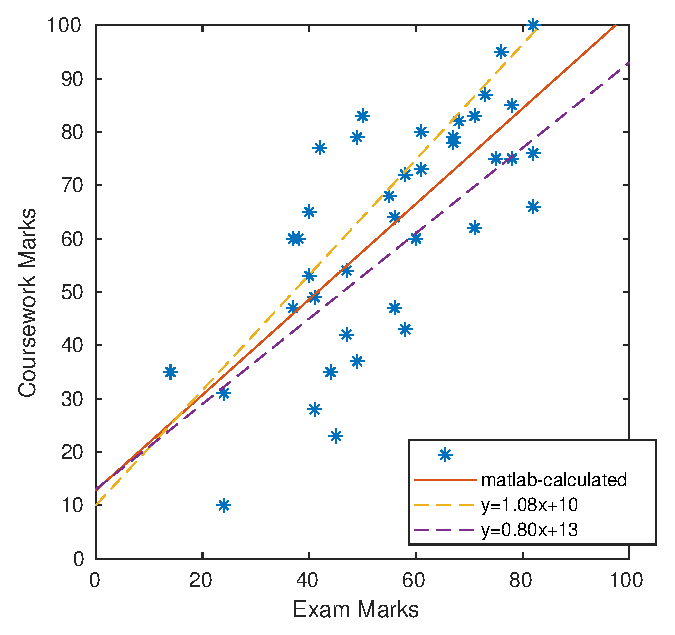
\includegraphics[scale=0.6, center]{./eps/topic1_c.eps}
	\caption{Coursework marks plotted against exam marks. }
	\label{fig:Topic1-c}
\end{figure}
Therefore the uncertainty in the parameters is
\begin{equation}
	content...
\end{equation}
\lstinputlisting[caption={Code for Topic 1. Question c.}]{"./files/topic 1/c.m"}

\subsection*{d}